\documentclass[a4paper,openright,12pt]{book}
\usepackage{graphicx}
% \usepackage{setspace}
\usepackage[sort&compress]{natbib}
\usepackage[spanish]{babel}
% \usepackage[utf8]{inputenc}
\usepackage{epsfig}
\usepackage{rotating}
\usepackage{amsmath}
\usepackage{slashbox}
\usepackage{setspace}
\usepackage{amsfonts}
\usepackage{dcolumn}
\usepackage{multirow}
\usepackage{url}
\usepackage{natbib}
\usepackage{amssymb}
\usepackage{times}
\usepackage{fontspec}
\usepackage{booktabs}
\usepackage{geometry}
\usepackage{cite}
\setcounter{secnumdepth}{3}
\setmainfont{Times New Roman}
\geometry{left=3cm,right=3cm,top=2.5cm,bottom=2.5cm}

\RequirePackage{ifpdf} % ¿latex o pdflatex?
% Configuración de las imágenes

\usepackage{graphicx}		% Inclusión de imágenes
\DeclareGraphicsExtensions{.eps}

\graphicspath{ {imgs/} } % Ruta respecto al fichero tex principal dónde se buscan imágenes

\onehalfspace
\begin{document}

\begin{titlepage}

\begin{center}
\vspace*{-1in}
\begin{figure}[htb]
\begin{center}

\includegraphics[height=2cm]{./imgs/logo_uz}
\hfill
\includegraphics[height=2cm]{./imgs/logo_fecem}
\end{center}
\end{figure}

FACULTAD DE CIENCIAS ECONÓMICAS Y EMPRESARIALES\\
\vspace*{0.15in}
DEPARTAMENTO DE ESTRUCTURA ECONÓMICA\\
\vspace*{0.6in}
\begin{large}
TRABAJO\\
\end{large}
\vspace*{0.2in}
\begin{Large}
\textbf{COMERCIO INTERNACIONAL} \\
\end{Large}
\vspace*{0.3in}
\begin{large}
Análisis de la economía de Chipre\\
\end{large}
\vspace*{0.3in}
%\rule{80mm}{0.1mm}\\
%\vspace*{0.1in}
\begin{large}
Autor: \\
Maximiliano Greco \\
\end{large}
\end{center}

\end{titlepage}

\newpage


\chapter{Presentación Del País}
\label{cap1}


Para este trabajo se me ha asignado analizar la economía de Chipre. Es un país europeo, con las coordenadas: 35°10′00″N 33°21′00″E que se corresponde con el suroeste asiático. Cómo puede verse en la Figura \ref{fig1} sin embargo, a pesar de su situación próxima a Asia, tanto política cómo culturalmente se lo considera europeo, además es un estado miembro de la Unión Europea y se trata de un país cuyo gobierno es Républica presidencialista, con capital de nombre Nicosia. Los idiomas oficiales son Griego y Turco.

\begin{figure}[htb]
    \centering
    \caption{Situación geográfica de Chipre}
    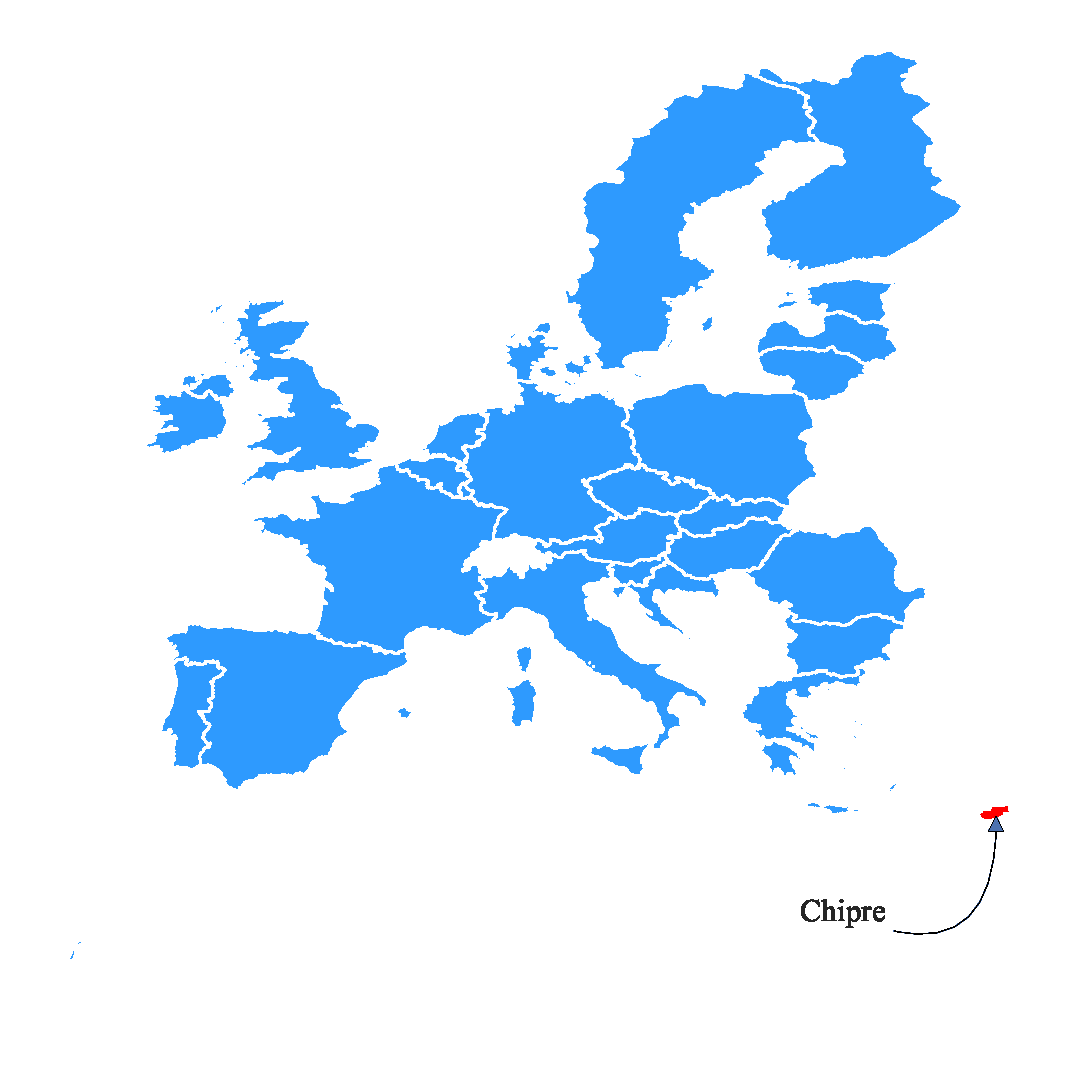
\includegraphics[width=300px]{imgs/mapa.eps}
    \label{fig1}
\end{figure}

Chipre posee recursos naturales como cobre, pirita, asbesto, yeso, madera, sal, mármol y tierra de arcilla.

Además de los anteriores, Chipre posee una relevante fuente de gas natural y petróleo que se encuentra actualmente en fase de exploración y análisis. Se estima que estos recursos se puedan empezar a explotar a partir de 2018-2020.



\chapter{Evolución Del Comercio}
\label{cap2}

% Please add the following required packages to your document preamble:
% \usepackage{booktabs}
\begin{table}[]
\centering
\caption{Evolución de la exportaciones de Chipre.}
\label{tab1}
\begin{tabular}{@{}lrr@{}}
\toprule
Año  & \multicolumn{1}{l}{\begin{tabular}[c]{@{}l@{}}Exportaciones de \\ bienes y servicios \\ (constante LCU)\end{tabular}} & \multicolumn{1}{l}{\begin{tabular}[c]{@{}l@{}}Exportaciones de \\ bienes y servicios \\ (corriente LCU)\end{tabular}} \\ \midrule
1980 & 2.022.014.400,00                                                                                                      & 587.929.800,00                                                                                                        \\
1981 & 2.306.751.300,00                                                                                                      & 752.126.400,00                                                                                                        \\
1982 & 2.489.220.600,00                                                                                                      & 891.719.100,00                                                                                                        \\
1983 & 2.692.482.800,00                                                                                                      & 979.028.600,00                                                                                                        \\
1984 & 3.099.007.700,00                                                                                                      & 1.248.987.700,00                                                                                                      \\
1985 & 3.065.484.100,00                                                                                                      & 1.234.293.700,00                                                                                                      \\
1986 & 3.013.713.800,00                                                                                                      & 1.231.901.600,00                                                                                                      \\
1987 & 3.426.603.700,00                                                                                                      & 1.438.300.700,00                                                                                                      \\
1988 & 3.890.415.000,00                                                                                                      & 1.639.573.900,00                                                                                                      \\
1989 & 4.540.090.700,00                                                                                                      & 1.984.369.800,00                                                                                                      \\
1990 & 4.843.499.200,00                                                                                                      & 2.248.861.100,00                                                                                                      \\
1991 & 4.433.579.400,00                                                                                                      & 2.151.812.500,00                                                                                                      \\
1992 & 5.314.100.000,00                                                                                                      & 2.622.019.800,00                                                                                                      \\
1993 & 5.163.456.700,00                                                                                                      & 2.657.217.000,00                                                                                                      \\
1994 & 5.586.530.600,00                                                                                                      & 2.974.675.100,00                                                                                                      \\
1995 & 6.527.120.000,00                                                                                                      & 5.126.300.000,00                                                                                                      \\
1996 & 6.934.680.000,00                                                                                                      & 5.602.220.000,00                                                                                                      \\
1997 & 6.938.190.000,00                                                                                                      & 5.793.210.000,00                                                                                                      \\
1998 & 7.320.920.000,00                                                                                                      & 6.223.840.000,00                                                                                                      \\
1999 & 7.507.970.000,00                                                                                                      & 6.512.990.000,00                                                                                                      \\
2000 & 8.167.940.000,00                                                                                                      & 7.412.550.000,00                                                                                                      \\
2001 & 8.345.640.000,00                                                                                                      & 7.787.330.000,00                                                                                                      \\
2002 & 8.004.010.000,00                                                                                                      & 7.411.900.000,00                                                                                                      \\
2003 & 7.892.310.000,00                                                                                                      & 7.419.710.000,00                                                                                                      \\
2004 & 8.088.910.000,00                                                                                                      & 7.882.900.000,00                                                                                                      \\
2005 & 8.254.850.000,00                                                                                                      & 8.254.850.000,00                                                                                                      \\
2006 & 8.359.440.000,00                                                                                                      & 8.549.730.000,00                                                                                                      \\
2007 & 8.800.990.000,00                                                                                                      & 9.326.470.000,00                                                                                                      \\ \bottomrule
\end{tabular}
\end{table}

\begin{figure}[htb]
    \caption{Evolución de las exportaciones ($Lambda$ \%) y su frecuencia.}
    \centering
    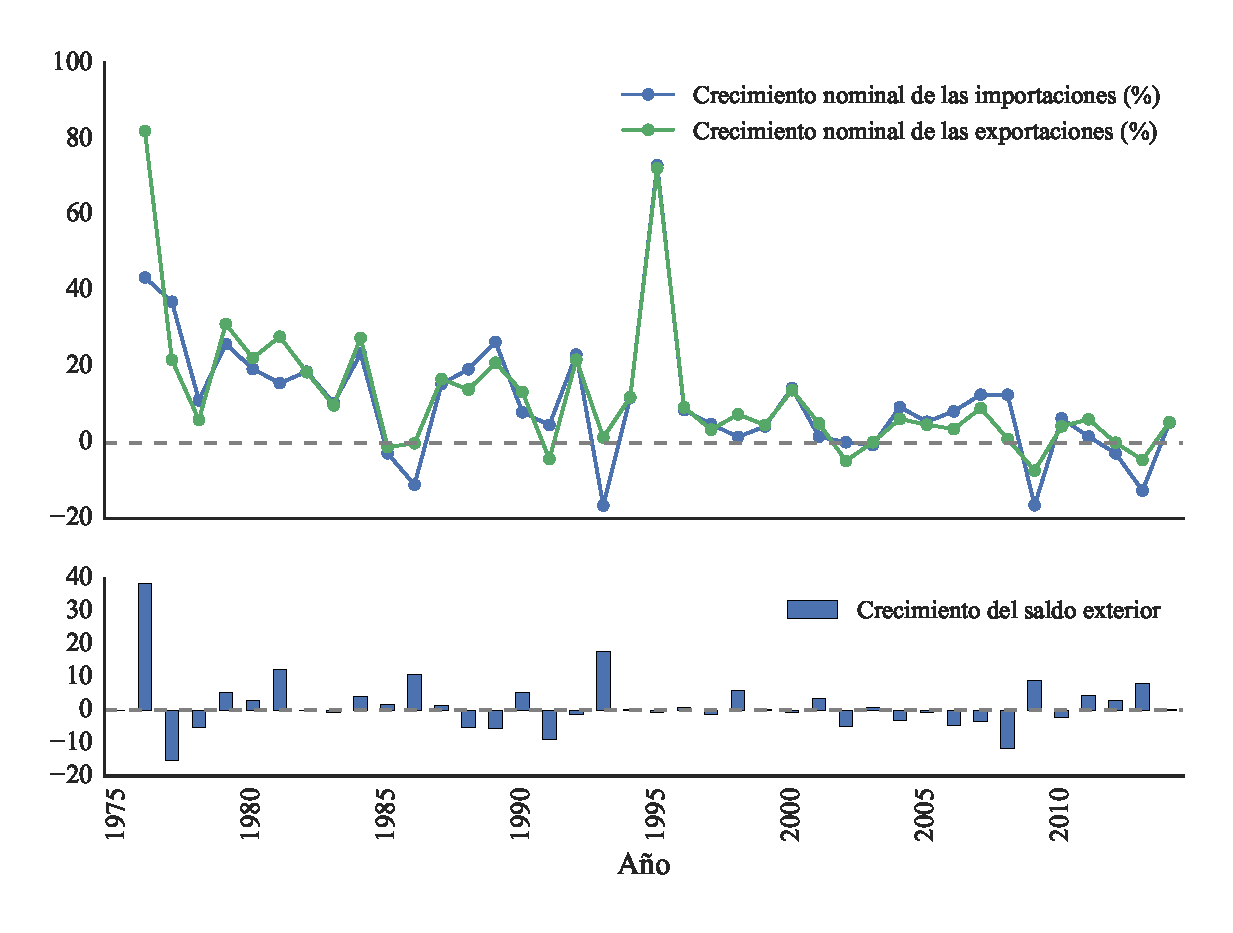
\includegraphics[width=300px]{imgs/ev_dx.eps}
    \label{ev_x}
\end{figure}




\begin{table}[]
\centering
\caption{Evolución de las importaciones de Chipre.}
\label{tab2}
\begin{tabular}{@{}lrr@{}}
\toprule
date & \multicolumn{1}{l}{\begin{tabular}[c]{@{}l@{}}Importaciones de \\ bienes y servicios \\ (constante LCU)\end{tabular}} & \multicolumn{1}{l}{\begin{tabular}[c]{@{}l@{}}Importaciones de \\ bienes y servicios \\ (corriente LCU)\end{tabular}} \\ \midrule
1980 & 2.676.118.100,00                                                                                                      & 819.274.400,00                                                                                                        \\
1981 & 2.743.072.900,00                                                                                                      & 947.761.300,00                                                                                                        \\
1982 & 3.094.066.300,00                                                                                                      & 1.124.943.200,00                                                                                                      \\
1983 & 3.264.572.800,00                                                                                                      & 1.242.495.000,00                                                                                                      \\
1984 & 3.798.964.600,00                                                                                                      & 1.533.298.900,00                                                                                                      \\
1985 & 3.626.378.900,00                                                                                                      & 1.489.900.500,00                                                                                                      \\
1986 & 3.229.223.700,00                                                                                                      & 1.324.507.800,00                                                                                                      \\
1987 & 3.688.343.200,00                                                                                                      & 1.529.027.400,00                                                                                                      \\
1988 & 4.176.573.800,00                                                                                                      & 1.824.615.500,00                                                                                                      \\
1989 & 5.015.381.800,00                                                                                                      & 2.308.833.100,00                                                                                                      \\
1990 & 5.302.331.700,00                                                                                                      & 2.493.703.900,00                                                                                                      \\
1991 & 5.407.130.200,00                                                                                                      & 2.609.205.300,00                                                                                                      \\
1992 & 6.403.969.100,00                                                                                                      & 3.214.904.500,00                                                                                                      \\
1993 & 5.226.227.600,00                                                                                                      & 2.681.479.100,00                                                                                                      \\
1994 & 5.597.598.500,00                                                                                                      & 2.999.449.800,00                                                                                                      \\
1995 & 6.531.110.000,00                                                                                                      & 5.192.630.000,00                                                                                                      \\
1996 & 6.842.650.000,00                                                                                                      & 5.636.820.000,00                                                                                                      \\
1997 & 6.926.900.000,00                                                                                                      & 5.909.750.000,00                                                                                                      \\
1998 & 6.963.940.000,00                                                                                                      & 5.998.680.000,00                                                                                                      \\
1999 & 7.133.060.000,00                                                                                                      & 6.255.730.000,00                                                                                                      \\
2000 & 7.790.250.000,00                                                                                                      & 7.155.010.000,00                                                                                                      \\
2001 & 7.775.370.000,00                                                                                                      & 7.265.740.000,00                                                                                                      \\
2002 & 7.747.590.000,00                                                                                                      & 7.273.030.000,00                                                                                                      \\
2003 & 7.672.140.000,00                                                                                                      & 7.224.510.000,00                                                                                                      \\
2004 & 8.205.030.000,00                                                                                                      & 7.900.090.000,00                                                                                                      \\
2005 & 8.333.830.000,00                                                                                                      & 8.333.840.000,00                                                                                                      \\
2006 & 8.809.070.000,00                                                                                                      & 9.019.310.000,00                                                                                                      \\
2007 & 9.730.760.000,00                                                                                                      & 10.159.530.000,00                                                                                                     \\ \bottomrule
\end{tabular}
\end{table}


\begin{figure}[htb]
    \caption{Evolución de las importaciones ($\Lambda$ \%) y su frecuencia.}
    \centering
    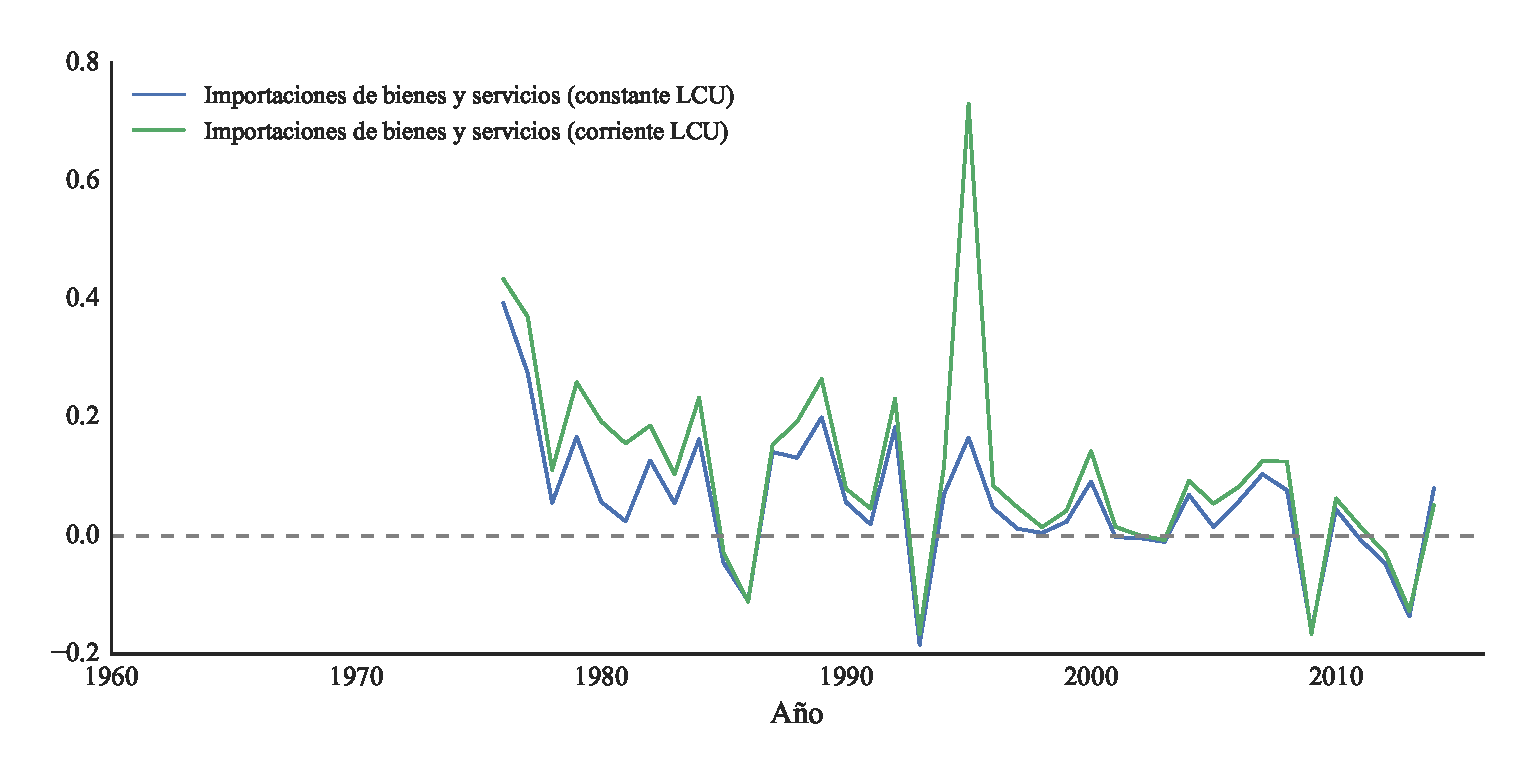
\includegraphics[width=300px]{imgs/ev_m.eps}
    \label{ev_m}
\end{figure}

La relación real de intercambio (RRI) es $RRI = \frac{P_x}{P_m} = \frac{IVU_x}{IVU_m} 100$ por tanto cuando la realación real de intercambio es mayor que 100 tenemos que el valor de las exportaciones son mayores que las importaciones y viceversa. Que la RRI sea mayor que 100 implica que para una mismca cantidad de exportaciones el país puede obtener una mayor cantidad de importaciones, lo cual mejora el bienestar es decir el comercio internacional reporta beneficios.

\begin{figure}[htb]
    \centering
    \caption{Relación Real de Intercambio de Chipre}
    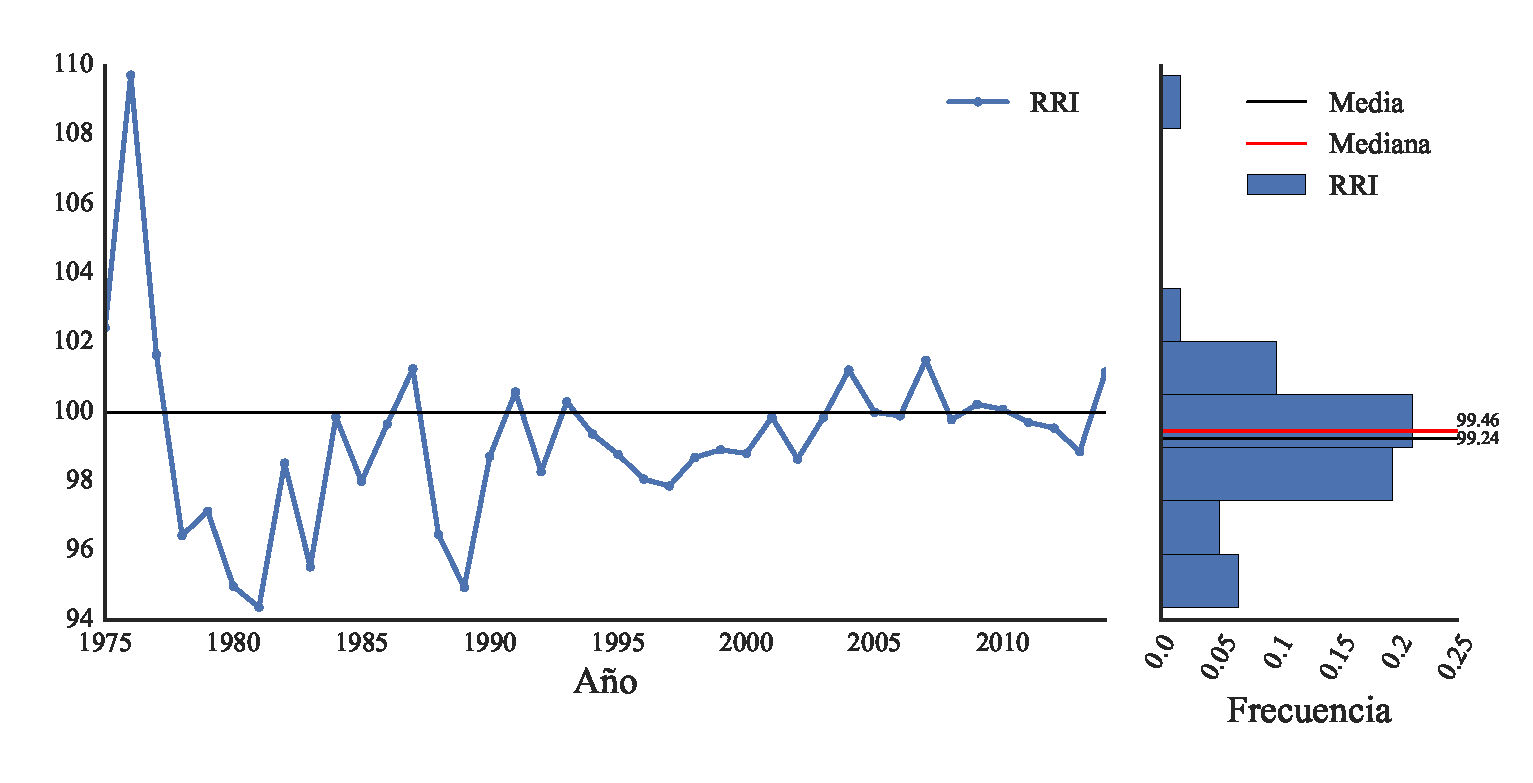
\includegraphics[width=300px]{imgs/rri_0.eps}
    \label{rri}
\end{figure}

Cómo puede verse en al Figura \ref{rri}, la evolución de la relación real de intercambio de Chipre, gira en torno a un valor por debajo del 100\%, aproximadamente 99.46\% es el porcentaje medio y 99.24\% es el valor de la mediana, como puede constatarse en el histograma de la derecha, mas del 50\% de las observaciones la RRI de chipre se hallan con valores inferiores al 99.24\%, esto estrictamente indica que Chipre pierde bienestar con el comercio internacional, dado que el valor de lo que importa es superior a lo que exporta, lo que implica que para una mismca cantidad de exportaciones cada vez puede importar menos. En el periodo analizado sin duda Chipre ha perdido bienestar con el comercio internacional con más frecuencia que el que ha ganado.

\chapter{Distribución Geográfica De M Y X}
\label{cap3}




\chapter{Competitividad Precio O Coste}
\label{cap4}

\chapter{Competitividad Estructural}
\label{cap5}

\chapter{Especialización comercial}

\chapter{Comercio Intraindustrial}

\chapter{Política Comercial}

\chapter{Resumen y Conclusiones}

\chapter{Anexo}

En el Capítulo \ref{cap1} se han usado los siguientes indicadores:

\begin{enumerate}

    \item BALANZA COMERCIAL

    $$X - M$$
    \item TASA DE COBERTURA

    $$\frac{X}{M}100$$
    \item PENETRACIÓN DE LAS IMPORTACIONES

    $$\frac{M}{\text{PIB} + M - X} 100$$
    \item GRADO DE APERTURA

    $$\frac{X+M}{\text{PIB}} 100$$
    \item PROPENSIÓN EXPORTADORA

    $$\frac{X}{\text{PIB}} 100$$

\end{enumerate}

Para el Capítulo \ref{cap3}:

\begin{enumerate}
    \item COMPETITIVIDAD PRECIO O COSTE
    \begin{enumerate}
        \item Indices de tipo de cambio efectivo real
        \item Tipo de cambio oficial
        \item Tasa de inflación
    \end{enumerate}

\item ESPECIALIZACIÓN COMERCIAL

\item  INDICE DE DEPENDENCIA

Para todo país $h$ y el sector $i$

$$IDep^h_i = \frac{\frac{M^h_i}{\sum_i M^h_i}}{\frac{\sum_h M^h_i}{\sum_h \sum_i M^h_i}} 100$$

\item  INDICE DE ESPECIALIZACIÓN

$$IEsp^h_i = \frac{\frac{X^h_i}{\sum_i X^h_i}}{\frac{\sum_h X^h_i}{\sum_h \sum_i X^h_i}} 100$$

\item  SALDO COMERCIAL RELATIVO

$$SCR_i = \frac{X_i - M_i}{X_i + M_i} 100$$

\item IMPORTANCIA RELATIVA DEL SECTOR EN LAS IMPORTACIONES Y EXPORTACIONES.

$$IRX_i = \frac{X_i}{\sum_i X_i}$$

$$IRM_i = \frac{M_i}{\sum_i M_i}$$

\item COMERCIO INTRAINDUSTRIAL

$$IGL_i = \frac{X_i + M_i - |X_i - M_i|}{X_i + M_i}100$$

$$IGL_{agg} = \frac{\sum_i(X_i + M_i) - \sum_i |X_i - M_i|}{\sum_i (X_i + M_i)}100$$

\end{enumerate}


\cleardoublepage
\addcontentsline{toc}{chapter}{Bibliografía}
\bibliographystyle{apalike}
\bibliography{biblio.bib} % yyyy.bib es el fichero donde está salvada la bibliografía.







\end{document}
